\documentclass{article}

% if you need to pass options to natbib, use, e.g.:
%     \PassOptionsToPackage{numbers, compress}{natbib}
% before loading neurips_2021

% ready for submission
\usepackage{neurips_2021}

% to compile a preprint version, e.g., for submission to arXiv, add add the
% [preprint] option:
%     \usepackage[preprint]{neurips_2021}

% to compile a camera-ready version, add the [final] option, e.g.:
%     \usepackage[final]{neurips_2021}

% to avoid loading the natbib package, add option nonatbib:
%    \usepackage[nonatbib]{neurips_2021}

\usepackage[utf8]{inputenc} % allow utf-8 input
\usepackage[T1]{fontenc}    % use 8-bit T1 fonts
\usepackage{hyperref}       % hyperlinks
\usepackage{url}            % simple URL typesetting
\usepackage{booktabs}       % professional-quality tables
\usepackage{amsfonts}       % blackboard math symbols
\usepackage{nicefrac}       % compact symbols for 1/2, etc.
\usepackage{microtype}      % microtypography
\usepackage{xcolor}         % colors


\usepackage{amsmath}
\usepackage{graphicx}
\usepackage{tikz}
\usetikzlibrary{bayesnet}
\newcommand{\prob}[1]{\operatorname{Pr}\left[\,#1\,\right]}   
\newcommand{\expect}[1]{\operatorname{E}\left[\,#1\,\right]}   
\def\cond{\; | \;}

\title{Variational Inference for Dirichlet Process to Stratify Cancer
Patients Using DNA Methylation}

% The \author macro works with any number of authors. There are two commands
% used to separate the names and addresses of multiple authors: \And and \AND.
%
% Using \And between authors leaves it to LaTeX to determine where to break the
% lines. Using \AND forces a line break at that point. So, if LaTeX puts 3 of 4
% authors names on the first line, and the last on the second line, try using
% \AND instead of \And before the third author name.

\author{%
  David S.~Hippocampus\thanks{Use footnote for providing further information
    about author (webpage, alternative address)---\emph{not} for acknowledging
    funding agencies.} \\
  Department of Computer Science\\
  Cranberry-Lemon University\\
  Pittsburgh, PA 15213 \\
  \texttt{hippo@cs.cranberry-lemon.edu} \\
  % examples of more authors
  % \And
  % Coauthor \\
  % Affiliation \\
  % Address \\
  % \texttt{email} \\
  % \AND
  % Coauthor \\
  % Affiliation \\
  % Address \\
  % \texttt{email} \\
  % \And
  % Coauthor \\
  % Affiliation \\
  % Address \\
  % \texttt{email} \\
  % \And
  % Coauthor \\
  % Affiliation \\
  % Address \\
  % \texttt{email} \\
}

\begin{document}

\maketitle

\begin{abstract}
Variational Inference (VI) is an alternative strategy to Markov Chain Monte Carlo (MCMC) which tends to be faster and easier to scale to larger datasets (Blei et al., 2016). This is especially advantageous in applications that interact with high dimensional data. Previous work has been done on a VI method for Dirichlet Process Mixture Models (DPMMs) based on the well-known stick-breaking process (Blei et al., 2016). In contrast, we propose a similar model, but based on the Chinese Restaurant Process (CRP) instead. This model has fewer parameters to estimate; therefore, we hypothesize that our model will perform faster than the model by Blei et al.
\\

DNA methylation is an epigenetic mark that is associated with transcriptional repression and may be closely related to cancer. A common objective is to identify a latent structure shared across cancers from different tissue types reflecting commonly altered gene pathways. These latent structures stratify cancer patients into functionally similar groups and can inform therapy decisions in clinical applications. This study will apply our VI model on DNA methylation data for stratification.  
\end{abstract}

\section{Introduction}


\subsection{DNA Methylation}

Cancers develop via the acquisition of genomic changes. These changes in turn alter the cells harbouring them, leading to changes in cell state (phenotype). One common effect of these mutations is to induce a series of modifications to the genome, which do not alter the encoded DNA but rather the ability of the DNA to be read and processed into protein. These heritable non-genetic changes are broadly referred to as epigenetic changes. According to Baylin and Jones (2011), "Epigenetic alterations are leading candidates for the development of specific markers for cancer detection, diagnosis and prognosis". One such epigenetic change is DNA methylation, which is unambiguously linked with transcriptional repression. When present in promoter regions, DNA methylation correlates negatively with gene expression; furthermore, characteristic changes in DNA methylation have been reported for cancer. Research indicates that gene promoter CpG islands acquire abnormal hypermethylation resulting in transcriptional silencing in cancer (Bock, 2012). It is important to note that 70-80\% of CpGs in the human genome are affected by DNA methylation. Therefore, understanding the effects of DNA methylation in cancer can provide valuable information for finding an effective remedy for cancer in humans. The potential relationship between DNA methylation and cancer opens up a new avenue of exploration. Advances in next-generation sequencing and microarray technology allow for analysis on DNA methylation in large samples and genome-wide; currently, DNA methylation is the only epigenetic mark that can be measured reliably. As a result, DNA methylation can be profiled accurately using high throughput sequencing and is a potential feature for categorizing cancer patients into functionally similar groups. 


\subsection{Variational Inference}

Variational inference is an alternative strategy to Markov Chain Monte Carlo (MCMC) sampling which tends to be faster and easier to scale to larger datasets (Blei et al., 2016). The key characteristic of variational inference is that it casts Bayesian inference as an optimization problem (Salimans et al., 2015). Variational inference attempts to approximate the posterior with another distribution $q_\theta(z|x)$ by choosing its parameters $\theta$ to optimize the evidence lower bound (ELBO) on the marginal likelihood,

%% I had to add the package amsmath, don't know if this is allowed...
\begin{align*}
\log{p(x)} &\geq \log p(x) - D_{KL}(q_\theta(z\mid x)||p(z\mid x))\\
		   &= E_{q_\theta(z\mid x)}(\log p(x,z)-\log q_\theta (z\mid x))
\end{align*}

In recent years, there have been many advances in the field of VI, which are summarized in a review by Zhang et al., (2019).

\subsection{Dirichlet Process and Chinese Restaurant Process}

The Dirichlet process is a stochastic process used for Bayesian nonparametric regression; in particular, for constructing Dirichlet process mixture models (Neal, 2000). A Dirichlet process $G$ is a distribution of distributions consisting of a base distribution $G_0$ and a positive real number $\alpha$, and can be written as, $G \sim \text{DP}(G_0, \alpha)$, where $G_0$ is a continuous distribution such that the probability of any two samples generated from this distribution being equal is zero, whereas $G$ is a discrete distribution consisting of infinitely many number of point masses,  so the probability of two samples colliding is non-zero.  For any measurable finite k partitions $\{B_i\}_{i=1}^k$,
\begin{align*}
G(B_1), \cdots, G(B_k))\sim \text{Dir}(\alpha G(B_1), \cdots, \alpha G(B_k))
\end{align*}
then
\begin{align*}
\prob{X_1, \cdots, X_k} = \int \prob{G} \prod_{i=1}^k \prob{X_i\cond G}\,dG
\end{align*}
which represents the dependencies among $\{X_i\}_{i=1}^k$ by marginalizing out $G$. \\

The Chinese restaurant process, stick-breaking process and Polya urn scheme are three common perspectives regarding the Dirichlet Process, and only the first method will be focused on in this project.  Assuming a restaurant has infinitely many tables,  and let $\{X_i\}_{i=1}^k$ be the customers of the restaurant.  Then $\{X_i\}_{i=1}^k$ are partitioned determined by the same table the represented customers sitting at.  Considering the behavior of $X_n$ given the previous $n-1$ observations:
\begin{align*}
X_n\cond (X_1 = x_1, X_2 = x_2, \cdots,  X_{n-1} = x_{n-1}) = \left\{
\begin{array}{rl}
x_n^* \, &\text{with probability}\ \frac{\cond\{j : x_j = n\}\cond}{n - 1 + \alpha}\\
\text{new draw from}\ G_0\, &\text{with probability}\  \frac{\alpha}{n - 1 + \alpha}
\end{array}
\right.
\end{align*}
where $\cond \{j: x_j = n\}\cond$ is the number of times the value $x_n$ occurs in $\{x_1, x_2, \cdots x_n\}$.


The fact is that people are more likely to sit at the tables where many people are already sitting, however,  the customers will sit at a new table with probability proportional to $\alpha$.\\

\subsection{Dirichlet Process Mixture Model}
The Dirichlet Process Mixture Model (DPMM) is the resulting hierarchical model of applying Dirichlet Process,  which was initially proposed for classifying data points into unbounded number of mixture components.  Given a sample from $\{x_1, \cdots, x_N\}$ from the DPMM,  the goal is to compute the posterior predictive distribution 
\begin{align*}
\prob{X = \hat{x}\cond x_1, \cdots, x_N, \alpha, G_0} = \int\prob{\hat{x}\cond x}\prob{x\cond x_1, \cdots, x_N, \alpha, G_0}\,dx,
\end{align*}
where the posterior distribution $\prob{x\cond x_1, \cdots, x_N}$ does not have a closed form.  The well-known EM algorithm is used for inference in finite by optimizing likelihood but for the finite mixture models,  so MCMC and Variational inference are better options as $G$ is nonparametric.

\section{Related Work}
Blei and Jordan (2006) provided a Variational inference algorithm for Dirichlet Process Mixture Models based on the stick-breaking process, and also compared the mean convergence time consumption among their proposed variational inference algorithm and MCMC (including Collapsed Gibbs sampler and Blocked Gibbs sampler).  Let the base distribution $G_0$ be
\begin{align*}
\prob{x^*\cond \lambda} = h(x^*)\exp(\lambda_1^\top x^* + \lambda_2(-a(x^*)) - a(\lambda))
\end{align*}
where $\lambda$s' are hyperparameters,  and $a(x^*)$ is a cumulant function.  Then the target function for prediction, which is constructed on the stick-breaking process, is 
\begin{align*}
\prob{x_n\cond z_n, x_1^*, x_2^*, \cdots} = \prod_{i=1}^\infty [h(x_n)\exp({x_i^*}^\top x_n - a(x_i^*))]^{\mathbf{1}[z_n = i]},
\end{align*}
However,  this is too complicated to directly compute with.  Variational Inference is brought up as an alternative,  along with the mean-field variational approximations assuming the independence of latent variables and a derived coordinate ascent algorithm,  resulting in a straightforward expression:
\begin{align*}
\prob{x_{N+1}\cond \ x_1, x_2, \cdots, x_{n-1}, \alpha, \lambda}\approx \sum_{t=1}^T \expect{\pi_t(\mathbf{v})}\expect{\prob{x_{N+1}\cond x_t^*}}
\end{align*}
where $q$ is an approximation to the predict distribution depending on $x_1, x_2, \cdots, \alpha, \lambda$,  and each component $v_i$ in $\mathbf{v}$ follows the beta distribution with parameters $(1, \alpha)$.
\section{Methods}
\label{gen_inst}
\subsection{Model}

We propose a Variational Inference Dirichlet Process Gaussian Mixture Model based on the Chinese Restaurant Process, to stratify cancer patients based on DNA methylation values. This paper will build upon Blei and Jordan's (2006) work on Variational Inference for Dirichlet Process Mixtures. Our method differs from theirs in that we base our model on a Chinese Restaurant Process as opposed to a stick-breaking process. This Variational Inference model will be implemented in the probabilistic programming language Pyro. See Figure 1 for the graphical models for each variant of the model.

\begin{figure}[!htp]
	\centering
	\begin{minipage}{0.45\textwidth}
		\centering
		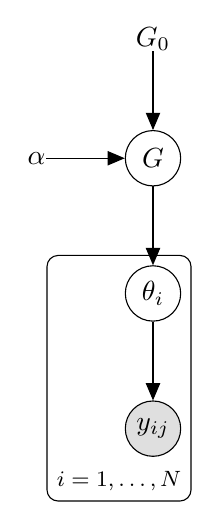
\begin{tikzpicture}
		  \node[obs] (y) {$y_{ij}$} ; % 
		  \node[latent, above=of y](theta){$\theta_i$} ; %
		  \node[latent, above=of theta] (G) {$G$} ; %
		  \node[const, above=of G] (G0) {$G_0$} ; %
		  \node[const, left=of G] (alpha) {$\alpha$} ; %
		
		  
		
		  \edge{G0}{G}
		  \edge{alpha}{G}
		  \edge{G}{theta}
		  \edge{theta}{y}
		  
		  
		  \plate {patients} { %
		    (y)(theta) %
		  } {$i=1,\ldots,N$} ; %
		\end{tikzpicture}
		\caption{Graphical model for DPMM based on CRP}
	\end{minipage}\hfill
	\begin{minipage}{0.45\textwidth}
		\centering
		\vspace{1.2cm}
		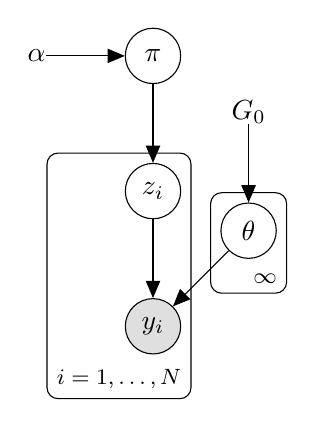
\begin{tikzpicture}
		  \node[obs] (y) {$y_{i}$} ; % 
		  \node[latent, above=of y] (z) {$z_i$} ; %
		  \node[latent, above=of z] (pi) {$\pi$} ; %
		  \node[const, left=of pi] (alpha) {$\alpha$} ; %
		  \node[latent, above right=of y] (theta) {$\theta$} ; %
		  \node[const, above=of theta] (G0) {$G_0$} ; %
		  
		
		  \edge{G0}{theta}
		  \edge{theta}{y}
		  \edge{z}{y}
		  \edge{pi}{z}
		  \edge{alpha}{pi}
		  
		  
		  \plate {patients} { %
		    (y)(z) %
		  } {$i=1,\ldots,N$} ; %
		  
		  \plate{clust_params}{
		   (theta)}{$\infty$}
		\end{tikzpicture}
		\caption{Graphical model for DPMM based on the stick-breaking process}
	\end{minipage}
\end{figure}


\subsection{Plots}
We intend to use clustermaps to visualize the main results, as our study is solving a clustering problem. Color bars on the left hand side indicates cancer type and purple squares represent the clusters. The more data points in the cluster, the larger the squares. The intensity of a square describes the proportion of iterations the data point of interest appeared in that cluster. We expect that the clustermaps in this study will resemble Figure 3, because data points should cluster by cancer types.

\begin{figure}[!htp]
	\centering
	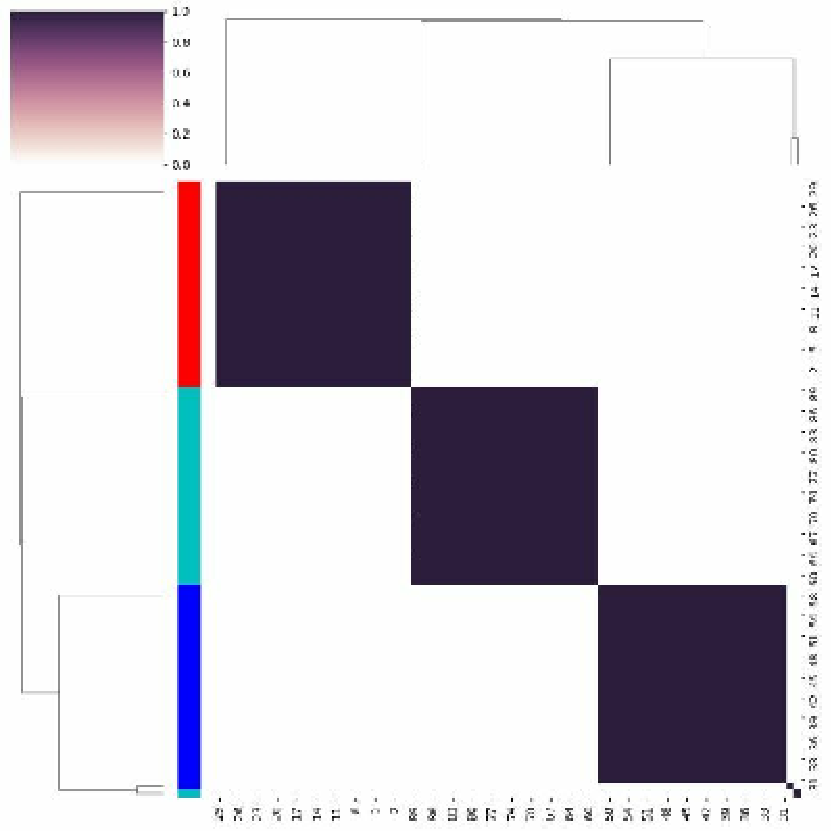
\includegraphics[scale=0.3]{figures/example_clustermap.pdf}
	\caption{Example of a clustermap. Color labels indicate cancer types: \color{red}{Type I}, \color{blue}{Type II}, \color{cyan}{Type III}}
\end{figure}


\section{Conclusion}
Variational Inference (VI) is an alternative strategy to Markov Chain Monte Carlo (MCMC) which tends to be faster and easier to scale to larger datasets (Blei et al., 2016). This is especially advantageous in applications that interact with high dimensional data, such as DNA methylation cluster analysis. We intend to build off the VI for DPMM model based on the stick-breaking process by Blei et al. and implement the same model, based on the Chinese Restaurant Process (CRP); the model will be written in the probabilistic programming language Pyro. We hypothesize that our model will be faster because it contains fewer parameters to estimate. Our model will be applied to a bioinformatic problem - stratifying cancer patients into functionally similar groups using DNA methylation. Consequently, these functionally similar groups can inform therapy decisions in clinical applications. 

\section*{References}

\medskip
{
\small

[1] Baylin, Stephen B., and Peter A. Jones.  A Decade of Exploring the Cancer Epigenome -- Biological and Translational Implications.  {\it Nature Reviews Cancer}, vol 11, no. 10, 23 Sept. 2011, pp. 726-734, 10.1038/nrc3130.

[2] Blei, David M, et al. Variational Inference: A Review for Statisticians. {\it Journal of the American Statistical Association}, vol. 112, no. 518, 27 Feb. 2017, pp. 859-877, arxiv.org/abs/1601.00670, 10.1080/01621459.2017.1285773.

[3] Blei, David M., and Michael I. Jordan. Variational Inference for Dirichlet Process Mixtures. {\it Bayesian Analysis}, vol.1, no.1, Mar.2006, pp. 121-143, 10.1214/06-ba104.

[4] Bock, Christoph, et al. Quantitative Comparison of Genome-Wide DNA Methylation Mapping Technologies. {\it Nature Biotechnology}, vol. 28, no. 10, 19 Sept. 2010, pp. 1106-1114, 10.1038/nbt.1681.

[5] Salimans, Tim, et al.  Markov Chain Monte Carlo and Variational Inference: Bridging the Gap. ArXiv: 1410.6460, 19 May 2015, arxiv.org/abs/1410.6460.

[6] Zhang, Cheng, et al. Advances in Variational Inference. {\it IEEE Transactions on Pattern Analysis and Machine Intelligence}, vol. 41, no. 8, 1 Aug. 2019, pp. 2008-2026, 10.1109/tpami.2018.2889774.
}

%% **************Remove this after***************
\newpage
\section{Headings: first level}
\label{headings}

All headings should be lower case (except for first word and proper nouns),
flush left, and bold.

First-level headings should be in 12-point type.

\subsection{Headings: second level}

Second-level headings should be in 10-point type.

\subsubsection{Headings: third level}

Third-level headings should be in 10-point type.

\paragraph{Paragraphs}

There is also a \verb+\paragraph+ command available, which sets the heading in
bold, flush left, and inline with the text, with the heading followed by 1\,em
of space.

\section{Citations, figures, tables, references}
\label{others}

These instructions apply to everyone.

\subsection{Citations within the text}

The \verb+natbib+ package will be loaded for you by default.  Citations may be
author/year or numeric, as long as you maintain internal consistency.  As to the
format of the references themselves, any style is acceptable as long as it is
used consistently.

The documentation for \verb+natbib+ may be found at
\begin{center}
  \url{http://mirrors.ctan.org/macros/latex/contrib/natbib/natnotes.pdf}
\end{center}
Of note is the command \verb+\citet+, which produces citations appropriate for
use in inline text.  For example,
\begin{verbatim}
   \citet{hasselmo} investigated\dots
\end{verbatim}
produces
\begin{quote}
  Hasselmo, et al.\ (1995) investigated\dots
\end{quote}

If you wish to load the \verb+natbib+ package with options, you may add the
following before loading the \verb+neurips_2021+ package:
\begin{verbatim}
   \PassOptionsToPackage{options}{natbib}
\end{verbatim}

If \verb+natbib+ clashes with another package you load, you can add the optional
argument \verb+nonatbib+ when loading the style file:
\begin{verbatim}
   \usepackage[nonatbib]{neurips_2021}
\end{verbatim}

As submission is double blind, refer to your own published work in the third
person. That is, use ``In the previous work of Jones et al.\ [4],'' not ``In our
previous work [4].'' If you cite your other papers that are not widely available
(e.g., a journal paper under review), use anonymous author names in the
citation, e.g., an author of the form ``A.\ Anonymous.''

\subsection{Footnotes}

Footnotes should be used sparingly.  If you do require a footnote, indicate
footnotes with a number\footnote{Sample of the first footnote.} in the
text. Place the footnotes at the bottom of the page on which they appear.
Precede the footnote with a horizontal rule of 2~inches (12~picas).

Note that footnotes are properly typeset \emph{after} punctuation
marks.\footnote{As in this example.}

\subsection{Figures}

\begin{figure}
  \centering
  \fbox{\rule[-.5cm]{0cm}{4cm} \rule[-.5cm]{4cm}{0cm}}
  \caption{Sample figure caption.}
\end{figure}

All artwork must be neat, clean, and legible. Lines should be dark enough for
purposes of reproduction. The figure number and caption always appear after the
figure. Place one line space before the figure caption and one line space after
the figure. The figure caption should be lower case (except for first word and
proper nouns); figures are numbered consecutively.

You may use color figures.  However, it is best for the figure captions and the
paper body to be legible if the paper is printed in either black/white or in
color.

\subsection{Tables}

All tables must be centered, neat, clean and legible.  The table number and
title always appear before the table.  See Table~\ref{sample-table}.

Place one line space before the table title, one line space after the
table title, and one line space after the table. The table title must
be lower case (except for first word and proper nouns); tables are
numbered consecutively.

Note that publication-quality tables \emph{do not contain vertical rules.} We
strongly suggest the use of the \verb+booktabs+ package, which allows for
typesetting high-quality, professional tables:
\begin{center}
  \url{https://www.ctan.org/pkg/booktabs}
\end{center}
This package was used to typeset Table~\ref{sample-table}.

\begin{table}
  \caption{Sample table title}
  \label{sample-table}
  \centering
  \begin{tabular}{lll}
    \toprule
    \multicolumn{2}{c}{Part}                   \\
    \cmidrule(r){1-2}
    Name     & Description     & Size ($\mu$m) \\
    \midrule
    Dendrite & Input terminal  & $\sim$100     \\
    Axon     & Output terminal & $\sim$10      \\
    Soma     & Cell body       & up to $10^6$  \\
    \bottomrule
  \end{tabular}
\end{table}

\section{Final instructions}

Do not change any aspects of the formatting parameters in the style files.  In
particular, do not modify the width or length of the rectangle the text should
fit into, and do not change font sizes (except perhaps in the
\textbf{References} section; see below). Please note that pages should be
numbered.

\section{Preparing PDF files}

Please prepare submission files with paper size ``US Letter,'' and not, for
example, ``A4.''

Fonts were the main cause of problems in the past years. Your PDF file must only
contain Type 1 or Embedded TrueType fonts. Here are a few instructions to
achieve this.

\begin{itemize}

\item You should directly generate PDF files using \verb+pdflatex+.

\item You can check which fonts a PDF files uses.  In Acrobat Reader, select the
  menu Files$>$Document Properties$>$Fonts and select Show All Fonts. You can
  also use the program \verb+pdffonts+ which comes with \verb+xpdf+ and is
  available out-of-the-box on most Linux machines.

\item The IEEE has recommendations for generating PDF files whose fonts are also
  acceptable for NeurIPS. Please see
  \url{http://www.emfield.org/icuwb2010/downloads/IEEE-PDF-SpecV32.pdf}

\item \verb+xfig+ "patterned" shapes are implemented with bitmap fonts.  Use
  "solid" shapes instead.

\item The \verb+\bbold+ package almost always uses bitmap fonts.  You should use
  the equivalent AMS Fonts:
\begin{verbatim}
   \usepackage{amsfonts}
\end{verbatim}
followed by, e.g., \verb+\mathbb{R}+, \verb+\mathbb{N}+, or \verb+\mathbb{C}+
for $\mathbb{R}$, $\mathbb{N}$ or $\mathbb{C}$.  You can also use the following
workaround for reals, natural and complex:
\begin{verbatim}
   \newcommand{\RR}{I\!\!R} %real numbers
   \newcommand{\Nat}{I\!\!N} %natural numbers
   \newcommand{\CC}{I\!\!\!\!C} %complex numbers
\end{verbatim}
Note that \verb+amsfonts+ is automatically loaded by the \verb+amssymb+ package.

\end{itemize}

If your file contains type 3 fonts or non embedded TrueType fonts, we will ask
you to fix it.

\subsection{Margins in \LaTeX{}}

Most of the margin problems come from figures positioned by hand using
\verb+\special+ or other commands. We suggest using the command
\verb+\includegraphics+ from the \verb+graphicx+ package. Always specify the
figure width as a multiple of the line width as in the example below:
\begin{verbatim}
   \usepackage[pdftex]{graphicx} ...
   \includegraphics[width=0.8\linewidth]{myfile.pdf}
\end{verbatim}
See Section 4.4 in the graphics bundle documentation
(\url{http://mirrors.ctan.org/macros/latex/required/graphics/grfguide.pdf})

A number of width problems arise when \LaTeX{} cannot properly hyphenate a
line. Please give LaTeX hyphenation hints using the \verb+\-+ command when
necessary.

\begin{ack}
Use unnumbered first level headings for the acknowledgments. All acknowledgments
go at the end of the paper before the list of references. Moreover, you are required to declare
funding (financial activities supporting the submitted work) and competing interests (related financial activities outside the submitted work).
More information about this disclosure can be found at: \url{https://neurips.cc/Conferences/2021/PaperInformation/FundingDisclosure}.

Do {\bf not} include this section in the anonymized submission, only in the final paper. You can use the \texttt{ack} environment provided in the style file to autmoatically hide this section in the anonymized submission.
\end{ack}

\section*{References}

References follow the acknowledgments. Use unnumbered first-level heading for
the references. Any choice of citation style is acceptable as long as you are
consistent. It is permissible to reduce the font size to \verb+small+ (9 point)
when listing the references.
Note that the Reference section does not count towards the page limit.
\medskip

{
\small

[1] Alexander, J.A.\ \& Mozer, M.C.\ (1995) Template-based algorithms for
connectionist rule extraction. In G.\ Tesauro, D.S.\ Touretzky and T.K.\ Leen
(eds.), {\it Advances in Neural Information Processing Systems 7},
pp.\ 609--616. Cambridge, MA: MIT Press.

[2] Bower, J.M.\ \& Beeman, D.\ (1995) {\it The Book of GENESIS: Exploring
  Realistic Neural Models with the GEneral NEural SImulation System.}  New York:
TELOS/Springer--Verlag.

[3] Hasselmo, M.E., Schnell, E.\ \& Barkai, E.\ (1995) Dynamics of learning and
recall at excitatory recurrent synapses and cholinergic modulation in rat
hippocampal region CA3. {\it Journal of Neuroscience} {\bf 15}(7):5249-5262.
}

%%%%%%%%%%%%%%%%%%%%%%%%%%%%%%%%%%%%%%%%%%%%%%%%%%%%%%%%%%%%
\section*{Checklist}

%%% BEGIN INSTRUCTIONS %%%
The checklist follows the references.  Please
read the checklist guidelines carefully for information on how to answer these
questions.  For each question, change the default \answerTODO{} to \answerYes{},
\answerNo{}, or \answerNA{}.  You are strongly encouraged to include a {\bf
justification to your answer}, either by referencing the appropriate section of
your paper or providing a brief inline description.  For example:
\begin{itemize}
  \item Did you include the license to the code and datasets? \answerYes{See Section~\ref{gen_inst}.}
  \item Did you include the license to the code and datasets? \answerNo{The code and the data are proprietary.}
  \item Did you include the license to the code and datasets? \answerNA{}
\end{itemize}
Please do not modify the questions and only use the provided macros for your
answers.  Note that the Checklist section does not count towards the page
limit.  In your paper, please delete this instructions block and only keep the
Checklist section heading above along with the questions/answers below.
%%% END INSTRUCTIONS %%%

\begin{enumerate}

\item For all authors...
\begin{enumerate}
  \item Do the main claims made in the abstract and introduction accurately reflect the paper's contributions and scope?
    \answerTODO{}
  \item Did you describe the limitations of your work?
    \answerTODO{}
  \item Did you discuss any potential negative societal impacts of your work?
    \answerTODO{}
  \item Have you read the ethics review guidelines and ensured that your paper conforms to them?
    \answerTODO{}
\end{enumerate}

\item If you are including theoretical results...
\begin{enumerate}
  \item Did you state the full set of assumptions of all theoretical results?
    \answerTODO{}
	\item Did you include complete proofs of all theoretical results?
    \answerTODO{}
\end{enumerate}

\item If you ran experiments...
\begin{enumerate}
  \item Did you include the code, data, and instructions needed to reproduce the main experimental results (either in the supplemental material or as a URL)?
    \answerTODO{}
  \item Did you specify all the training details (e.g., data splits, hyperparameters, how they were chosen)?
    \answerTODO{}
	\item Did you report error bars (e.g., with respect to the random seed after running experiments multiple times)?
    \answerTODO{}
	\item Did you include the total amount of compute and the type of resources used (e.g., type of GPUs, internal cluster, or cloud provider)?
    \answerTODO{}
\end{enumerate}

\item If you are using existing assets (e.g., code, data, models) or curating/releasing new assets...
\begin{enumerate}
  \item If your work uses existing assets, did you cite the creators?
    \answerTODO{}
  \item Did you mention the license of the assets?
    \answerTODO{}
  \item Did you include any new assets either in the supplemental material or as a URL?
    \answerTODO{}
  \item Did you discuss whether and how consent was obtained from people whose data you're using/curating?
    \answerTODO{}
  \item Did you discuss whether the data you are using/curating contains personally identifiable information or offensive content?
    \answerTODO{}
\end{enumerate}

\item If you used crowdsourcing or conducted research with human subjects...
\begin{enumerate}
  \item Did you include the full text of instructions given to participants and screenshots, if applicable?
    \answerTODO{}
  \item Did you describe any potential participant risks, with links to Institutional Review Board (IRB) approvals, if applicable?
    \answerTODO{}
  \item Did you include the estimated hourly wage paid to participants and the total amount spent on participant compensation?
    \answerTODO{}
\end{enumerate}

\end{enumerate}

%%%%%%%%%%%%%%%%%%%%%%%%%%%%%%%%%%%%%%%%%%%%%%%%%%%%%%%%%%%%

\appendix

\section{Appendix}

Optionally include extra information (complete proofs, additional experiments and plots) in the appendix.
This section will often be part of the supplemental material.

\end{document}